\documentclass[UTF-8,zihao=-4]{ctexart}

% --- 基础宏包 ---
\usepackage{geometry} % 设置页边距
\usepackage{graphicx} % 插入图片
\usepackage{amsmath} % 数学公式
\usepackage{amssymb} % 数学符号
\usepackage{float} % 控制图表浮动位置, [H]表示强制在此处
\usepackage{hyperref} % 生成超链接
\usepackage{listings} % 插入代码
\usepackage{xcolor} % 定义颜色
\usepackage{booktabs} % 三线表宏包
\usepackage{tabularx} % 等宽表格
\usepackage{fancyhdr} % 自定义页眉页脚
\usepackage{caption} % 图表标题格式定制
\usepackage{array} % 表格列格式

% --- 表格内容居中的 X 列类型 ---
\newcolumntype{C}{>{\centering\arraybackslash}X}

% --- 字体设置 ---
\setCJKmainfont{SimSun}[BoldFont=SimHei]  % 宋体正文，加粗映射到黑体
\setCJKsansfont{SimHei}                   % 黑体，用于标题
\setmainfont{Times New Roman}              % 新罗马，英文/数字

% --- 页面设置 ---
\geometry{a4paper, left=2.5cm, right=2.5cm, top=3cm, bottom=2.5cm}
\setlength{\baselineskip}{22pt} % 正文行距固定值22磅

% --- 标题格式设置 ---
% 一级标题 (1.)：黑体四号，大间距突出
% 二级标题 (1.1)：黑体小四，中间距
% 三级标题 (1.1.1)：黑体小四，紧贴正文
\ctexset{
    section = {
        format = {\heiti\zihao{4}},
        aftername = {\quad},
        beforeskip = {14pt},
        afterskip = {8pt},
    },
    subsection = {
        format = {\heiti\zihao{-4}},
        aftername = {\quad},
        beforeskip = {10pt},
        afterskip = {5pt},
    },
    subsubsection = {
        format = {\heiti\zihao{-4}},
        aftername = {\quad},
        beforeskip = {6pt},
        afterskip = {2pt},
    },
}

% --- 图表标题格式：黑体/新罗马5号加粗 ---
\DeclareCaptionFont{wuhao}{\zihao{5}}
\captionsetup{
    font = {wuhao, bf},
    labelfont = {wuhao, bf},
    textfont = {wuhao, bf},
}

% --- 超链接设置 ---
\hypersetup{
    colorlinks=true,
    linkcolor=black,
    filecolor=magenta,
    urlcolor=blue,
    citecolor=black,
}

% --- 页眉页脚设置 ---
\pagestyle{fancy}
\fancyhf{}
\renewcommand{\headrulewidth}{0pt}
\rfoot{\thepage}

% --- 代码块样式定义 ---
\definecolor{codegreen}{rgb}{0,0.6,0}
\definecolor{codegray}{rgb}{0.5,0.5,0.5}
\definecolor{codepurple}{rgb}{0.58,0,0.82}
\definecolor{backcolour}{rgb}{0.95,0.95,0.92}

\lstdefinestyle{mystyle}{
    backgroundcolor=\color{backcolour},
    commentstyle=\color{codegreen},
    keywordstyle=\color{magenta},
    numberstyle=\tiny\color{codegray},
    stringstyle=\color{codepurple},
    basicstyle=\ttfamily\footnotesize,
    breakatwhitespace=false,
    breaklines=true,
    captionpos=b,
    keepspaces=true,
    numbers=left,
    numbersep=5pt,
    showspaces=false,
    showstringspaces=false,
    showtabs=false,
    tabsize=2
}
\lstset{style=mystyle}

%================================================
%==============  文档开始  ======================
%================================================
\begin{document}

% --- 扉页（封面）---
\thispagestyle{empty}

\begin{center}
    \vspace*{2cm}

    {\heiti\zihao{3} 作品E：送药小车}

    \vfill

    
\includegraphics[width=0.55\linewidth]{../pic/电赛logo.png}

    \vfill

    {\songti\zihao{4} 2026年8月}

    \vspace{2cm}

\end{center}

\newpage

% --- 摘要 ---
\thispagestyle{empty}

\noindent
{\zihao{-4}\textbf{摘要：}}{\zihao{-4}
本项目围绕智能送药小车系统展开，旨在实现自主循迹、病房号识别、定点停靠与双车协同作业功能。系统两辆车分别以香橙派与树莓派搭载MSPM0G3507为核心控制器，采用摄像头配合OpenCV实现高精度路径循迹，实时采集图像识别路口与病房号。算法层面，通过霍夫直线检测融合PID控制算法实现循迹平稳性与速度优化，基于YOLO11n模型实现病房号字符识别。系统完整实现了全部任务要求：单小车分别运送药品至近端、中部或远端病房并返回；双车协同运送至同一中部病房及不同远端病房送取药品。测试结果表明系统设计合理、算法有效、硬件稳定，各项指标满足题目要求。
}

\vspace{1cm}

\noindent
{\zihao{-4}\textbf{关键词：}}{\zihao{-4} 智能送药小车 PID控制算法 YOLO11n模型 双车协同控制}

\newpage

% --- 目录页（不标页码）---
\thispagestyle{empty}
\tableofcontents
\newpage

% --- 从正文开始标页码 ---
\setcounter{page}{1}

%================================================
%==============  正文部分  ======================
%================================================

\section{系统方案设计}

\subsection{方案论证与选择}

\subsubsection{巡线方案}

方案一：视觉巡线方案。

该方案优点是输出的方位为模拟量，并且黑线判断算法对白布黑点有过滤作用，受到的环境干扰更小；缺点是摄像头检测的黑线位置与当前小车所在黑线的位置有偏差，并且黑线检测-串口发送位置参数过程有时间间隔，导致即时性不足，同时小车过弯时摄像头可能丢线，导致小车跑偏。

方案二：光电对管巡线方案。

该方案优点是专注于黑线巡线，处理速度快，具有即时性；缺点是极容易受到光照、地面环境的干扰，需要做更多滤波算法。

方案比较与选择：考虑到本次地图巡的是红线不是标准的黑线并且路上有病房号可能造成干扰。因此方案选择方案一：视觉巡线方案。

\subsubsection{视觉模块设计方案}

方案一：树莓派4B方案。该方案优点是成本较低，功耗较低；缺点是CPU性能偏弱，巡线难以跑到较高的帧率，且无NPU，运行YOLO模型十分吃力。

方案二：香橙派5Pro方案。该方案优点是CPU性能强，巡线轻松满帧率，且拥有NPU，运行YOLO从容且精度高；缺点是成本较高，目前仍在持续涨价，且体积相对较大。

方案比较与选择：鉴于两辆小车的性能需求，选择香橙派5Pro作为小车1的视觉处理器，树莓派4B作为小车2的视觉处理器。

\subsubsection{机械设计方案}

方案一：沿底板环形叠放方案。该方案优点是小车重心低，运行稳定；缺点空间冗余较小，一旦长宽偏大运行过程容易过边界黑线。

方案二：向上垂直叠放方案。该方案优点空间冗余较充足，容易控制住长宽；缺点是小车重心较高。

方案比较与选择：基于题目对碰边界线的限制比较严格，同时考虑本项目对速度要求不是太高，最终选定方案二。

\subsection{总体方案描述}

本智能送药小车采用"视觉巡线为主，双核协同决策"的架构设计。其核心运行原理是：通过搭载于车体上方的摄像头实时采集地面图像，经视觉处理器运行图像处理算法，检测走廊红实线的位置偏差并识别病房号数字，同时通过串口将偏差量与路径决策下发至底层运动控制板，控制板据此驱动电机实现循迹行驶与转向动作，保证了小车循迹的准确性与任务执行的智能性；同时，视觉系统并行完成病房号数字的识别与读取，根据识别结果决策目标路径与转向策略，并通过无线通信模块实现双车之间的指令交互与状态同步，从而完成复杂的协同作业。两者分工明确，兼顾了巡线的实时性与视觉识别的智能性。系统架构如图\ref{fig:system_arch}所示。

\begin{figure}[H]
    \centering
    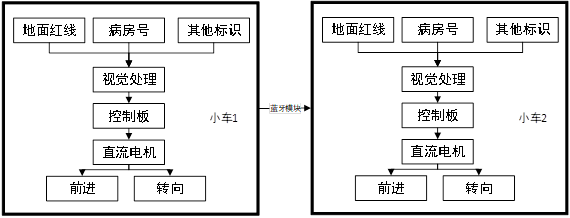
\includegraphics[width=0.85\linewidth]{../pic/system_arch.png}
    \caption{总体方案描述示意图}
    \label{fig:system_arch}
\end{figure}

\section{理论分析与计算}

\subsection{摄像头配合PID巡线原理}

视觉巡线原理：使用HSV提取图像中红线所在位置，随后使用霍夫直线检测得出摄像头图像内所有线段的起点、终点、斜率等信息，随后综合进行处理和线段筛选，剔除过短的线段和斜率过低的线段，得出巡线所需的偏移角度以及偏移中心的距离值。

\subsection{电机控制原理}

本系统采用双电机独立驱动架构，通过MSPM0G3507控制板的PWM输出实现电机转速调节。电机控制采用增量式PID算法，以编码器反馈的脉冲数作为速度反馈量，实时计算PWM占空比调整值。控制周期设为20ms，通过定时器中断实现精确时序，保证电机响应的即时性与稳定性。增量式PID控制算法如式\ref{eq:pid}所示：

\begin{equation} \label{eq:pid}
    \Delta u(k) = K_p \left[ e(k) - e(k-1) \right] + K_i e(k) + K_d \left[ e(k) - 2e(k-1) + e(k-2) \right]
\end{equation}

其中，$e(k)$ 为第 $k$ 次采样时的速度偏差，$K_p$、$K_i$、$K_d$ 分别为比例、积分、微分系数，$\Delta u(k)$ 为PWM占空比的增量调整值。

\section{电路与程序设计}

\subsection{电路设计分析}

\subsubsection{主电路设计}

主电路集成树莓派4B（或香橙派5Pro）、MSPM0G3507、OLED显示屏、JDY31/JDY34蓝牙模块、MPU6050陀螺仪、电机接口、调试接口等，板上集成三个降压模块，12V转5V给树莓派/香橙派供电，12V转3.3V给主控、传感器等供电，以及一个可变降压模块作为备用。

\subsubsection{电路板供电设计}

电路中使用了三个降压模块进行供电，产生三路不同电压等级的电压。电路中需要将5V电源提供给树莓派/香橙派，故在电路板中加入USB Type-C接口，保证供电能力的同时占用较小空间。供电逻辑如图\ref{fig:power}所示：

\begin{figure}[H]
    \centering
    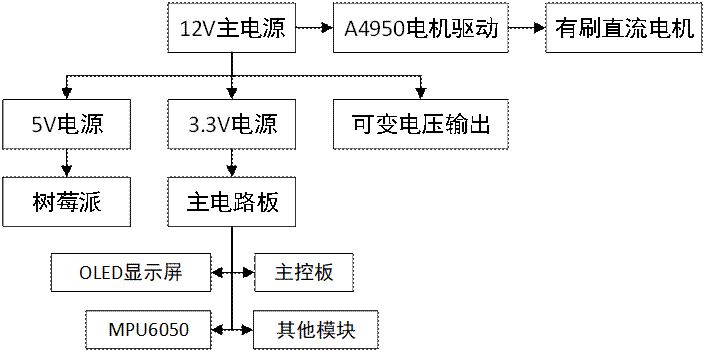
\includegraphics[width=0.7\linewidth]{../pic/image_2.png}
    \caption{基础供电逻辑图}
    \label{fig:power}
\end{figure}

\subsection{控制程序设计}

\subsubsection{底盘逻辑}

使用编码器读取电机单位时间（20ms）改变的脉冲数，进而得到电机速度，从而控制小车实现位置改变。

\subsubsection{巡线逻辑}

使用香橙派视觉模块实时采集赛道图像，计算黑线相对车体的横向偏移量（line\_x），通过串口发送至MSPM0G3507主控板。主控板将该偏移量作为PID巡线算法的输入，计算两电机速度差，实现基于视觉偏差的差速巡线控制。

\subsubsection{交叉路口识别与转向逻辑}

使用香橙派视觉模块进行交叉路口检测，通过解析串口传来的Road\_y（纵向位置）和isRoad\_T（T字路口标识）参数判断路口类型。当Road\_y超过阈值时识别为十字路口，当isRoad\_T为真时识别为T字路口。根据预设的路线栈和目标病房号，按照状态机逻辑选择转向方向，实现自主导航。

\subsubsection{控制逻辑}

小车与香橙派（树莓派）通过串口进行通信，采用自定义Hex协议传输数据。数据包包含Pos\_x（位置偏差）、line\_x（巡线偏差）、Road\_y（纵向位置）、Oran\_Num（识别到的数字）、isRoad\_T（T字路口标识）等信息。主控根据这些视觉参数控制电机进行相应的状态改变。

\subsubsection{OLED交互式菜单设计}

使用OLED进行参数改变和验收题目选择，实现便捷交互。

\subsection{视觉程序设计}

巡线部分使用OpenCV进行图像处理，使用HSV阈值提取出地面小车的行进轨迹线，随后使用霍夫直线检测拟合线段得出小车的偏移值以及地面轨迹线的斜率等，由线段斜率信息可进行对路口的判断以及位置的识别。同样使用HSV阈值提取地面的黑色像素，对提取出的图片进行轮廓检测，筛选出符合条件大小的轮廓，若轮廓数量达到一定值后判断为终点，并将这些轮廓用面积加权平均的方式得出终点的坐标值，便于定点停车。

药房的字符识别使用YOLO11n模型进行识别。由于识别目标特征较为突出，但是图像的采集条件较为恶劣，包括了高速移动、光照变化、目标被遮挡、弄脏、无法被摄像头捕捉完全等情况，因此在模型训练时采用了多种增强方式，在训练阶段对运动模糊、摄像头噪声、光照变化、遮挡、拍摄角度变化等情况进行的数据增强。树莓派方面情况更为特殊，将模型输入分辨率由640降为224，且输入图像转为灰度图，在图像预处理阶段对图像进行自适应直方图均衡化后再进行模型推理，以便突出特征，增强对比度。

数据传输任务采用pyserial库以及TCP协议与外界进行通信。pyserial库驱动串口与主控发送消息，为主控提供关键的视觉数据，TCP协议则是便于与电脑连接，大大提高了调试的便利性。

由于任务的复杂性，程序采用多文件、多进程结构，图像采集和巡线、字符检测以及数据传输分别采用单独进程运行，避免任务之间相互阻塞。进程间采用Pipe和SharedMemory进行数据传输，确保进程间通信正常。多个文件最终集合在单个程序中统一调度处理，同时方便使用systemd进行开机自启。视觉程序流程如图\ref{fig:vision_flow}所示。

\begin{figure}[H]
    \centering
    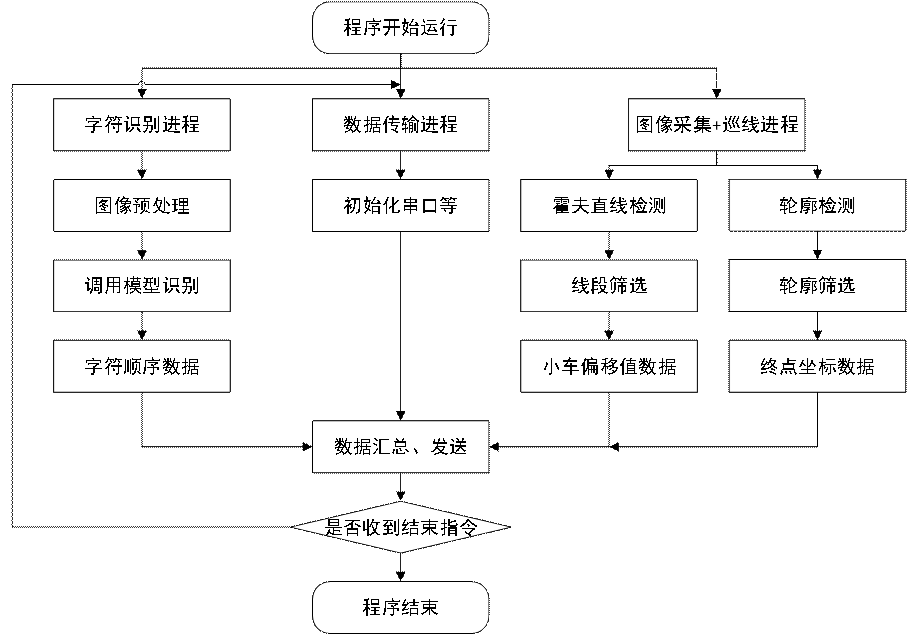
\includegraphics[width=0.6\linewidth]{../pic/image_3.png}
    \caption{视觉程序流程图}
    \label{fig:vision_flow}
\end{figure}

串口波特率设置为115200保证传输速度。

\section{设计报告测试方案与测试结果}

\subsection{测试环境}

测试环境如下表\ref{tab:test_env}所示：

\begin{table}[H]
    \centering
    \begin{tabularx}{\textwidth}{CC}
        \toprule
        测试器件名称 & 测试器件说明 \\
        \midrule
        秒表 & 用于测量小车总行驶时间 \\
        卷尺 & 用于测量小车尺寸 \\
        12V电池 & 用于为电机供电 \\
        OLED & 用于选择任务与查看参数 \\
        \bottomrule
    \end{tabularx}
    \caption{测试环境}
    \label{tab:test_env}
\end{table}

\subsection{测试方案}

\begin{enumerate}
    \item 步骤1：测量小车尺寸。
    \item 步骤2：将小车放在药房处（车头投影在门口区域内，面向病房），按要求1由测试专家指定一近端病房（1,2）号使小车识别对应数字运送药品到该病房，卸载药品后返回。测量小车行驶时间，观察小车行驶过程投影是否压线以及指示灯是否按要求正常变化。
    \item 步骤3：将小车放在药房处（车头投影在门口区域内，面向病房），按要求2由测试专家指定一中部病房号（3，4）使小车识别对应数字运送药品到该病房，卸载药品后返回。测量小车行驶时间，观察小车行驶过程投影是否压线以及指示灯是否按要求正常变化。
    \item 步骤4：将小车放在药房处（车头投影在门口区域内，面向病房），按要求3由测试专家指定一远端病房号（5,6,7,8）使小车识别对应数字运送药品到该病房，卸载药品后返回。测量小车行驶时间，观察小车行驶过程投影是否压线以及指示灯是否按要求正常变化。
    \item 步骤5：将小车放在药房处（车头投影在门口区域内，面向病房），由测试专家指定一中部病房号（3，4），使小车1,2识别对应数字并按要求4协同运送至该病房。测量小车行驶时间，观察小车行驶过程投影是否压线以及指示灯是否按要求正常变化。
    \item 步骤6：将小车放在药房处（车头投影在门口区域内，面向病房），由测试专家指定两个远端病房号（5,6,7,8），使小车1,2分别识别对应数字并按要求5协同取送药品至对应病房。测量小车行驶时间，观察小车行驶过程投影是否压线以及指示灯是否按要求正常变化。
\end{enumerate}

\subsection{测试结果与数据}

\subsubsection{小车尺寸测量结果}

小车尺寸测量结果如表\ref{tab:size}所示：

\begin{table}[H]
    \centering
    \begin{tabularx}{\textwidth}{CCCC}
        \toprule
        测试序号 & 长 $a$/cm & 宽 $b$/cm & 高 $c$/cm \\
        \midrule
        1 & 21.57 & 14.72 & 23.81 \\
        \bottomrule
    \end{tabularx}
    \caption{小车尺寸测试结果}
    \label{tab:size}
\end{table}

\subsubsection{要求1测试结果}

将小车放在路径的起始位置，运送药品至近端病房。测量小车行驶时间，观察小车行驶过程投影是否压线以及指示灯是否按要求正常变化，测试结果如表\ref{tab:task1}所示。

\begin{table}[H]
    \centering
    \begin{tabularx}{\textwidth}{CCCC}
        \toprule
        测试病房号 & 行驶总时间 $t$/s & 是否压线 & 指示灯是否按要求变化 \\
        \midrule
        1 & 9.33 & 否 & 是 \\
        2 & 9.27 & 否 & 是 \\
        \bottomrule
    \end{tabularx}
    \caption{要求1测试结果（近端病房）}
    \label{tab:task1}
\end{table}

\subsubsection{要求2测试结果}

将小车放在路径的起始位置，运送药品至中部病房。测量小车行驶时间，观察小车行驶过程投影是否压线以及指示灯是否按要求正常变化，测试结果如表\ref{tab:task2}所示。

\begin{table}[H]
    \centering
    \begin{tabularx}{\textwidth}{CCCC}
        \toprule
        测试病房号 & 行驶总时间 $t$/s & 是否压线 & 指示灯是否按要求变化 \\
        \midrule
        3 & 12.45 & 否 & 是 \\
        4 & 12.81 & 否 & 是 \\
        \bottomrule
    \end{tabularx}
    \caption{要求2测试结果（中部病房）}
    \label{tab:task2}
\end{table}

\subsubsection{要求3测试结果}

将小车放在路径的起始位置，运送药品至远端病房。测量小车行驶时间，观察小车行驶过程投影是否压线以及指示灯是否按要求正常变化，测试结果如表\ref{tab:task3}所示。

\begin{table}[H]
    \centering
    \begin{tabularx}{\textwidth}{CCCC}
        \toprule
        测试病房号 & 行驶总时间 $t$/s & 是否压线 & 指示灯是否按要求变化 \\
        \midrule
        5 & 18.86 & 否 & 是 \\
        6 & 18.93 & 否 & 是 \\
        7 & 17.99 & 否 & 是 \\
        8 & 18.37 & 否 & 是 \\
        \bottomrule
    \end{tabularx}
    \caption{要求3测试结果（远端病房）}
    \label{tab:task3}
\end{table}

\subsubsection{要求4测试结果}

将小车1,2放在路径的起始位置，协同运送药品至中部病房。测量小车1返回到药房且小车2到达病房的总时间（不包括小车2黄灯亮时的暂停时间），观察小车行驶过程投影是否压线以及指示灯是否按要求正常变化，测试结果如表\ref{tab:task4}所示。

\begin{table}[H]
    \centering
    \begin{tabularx}{\textwidth}{CCCC}
        \toprule
        测试病房号 & 行驶总时间 $t$/s & 是否压线 & 指示灯是否按要求变化 \\
        \midrule
        3 & 15.49 & 否 & 是 \\
        4 & 15.83 & 否 & 是 \\
        \bottomrule
    \end{tabularx}
    \caption{要求4测试结果（双车协同至同一中部病房）}
    \label{tab:task4}
\end{table}

\subsubsection{要求5测试结果}

将小车1,2放在路径的起始位置，协同取送药品至远端病房。测量小车1返回开始，到小车1返回到药房且小车2到达取药病房的总时间，观察小车行驶过程投影是否压线以及指示灯是否按要求正常变化，测试结果如表\ref{tab:task5}所示。

\begin{table}[H]
    \centering
    \begin{tabularx}{\textwidth}{CCCCC}
        \toprule
        \multicolumn{2}{>{\hsize=\dimexpr2\hsize+2\tabcolsep\relax}C}{测试病房号} & 行驶总时间 $t$/s & 是否压线 & 指示灯是否按要求变化 \\
        \cmidrule(lr){1-2}
        小车1 & 小车2 & & & \\
        \midrule
        5 & 8 & 23.56 & 否 & 是 \\
        6 & 7 & 23.79 & 否 & 是 \\
        \bottomrule
    \end{tabularx}
    \caption{要求5测试结果（双车协同至不同远端病房）}
    \label{tab:task5}
\end{table}

\subsection{测试结果分析}

根据测试所得数据，小车能够以较快的速度稳定行驶，准确识别病房号并运送药品至指定病房，基本符合预设要求；在后续双小车协同控制中，不同小车也能精准完成各自的任务，准确进行信息交换，并做出正确的行驶与停车响应，整体表现出较好的场地适应性与功能稳定性。各项测试中均未出现压线情况，指示灯变化均符合要求规范，行驶时间控制在合理范围内。系统整体运行稳定，满足题目各项指标要求。

\end{document}
